
\section{Synthesis and Future Directions}
\label{sec:conclusion}

This comprehensive survey establishes a unified framework for understanding implicit and explicit feedback in recommender systems, synthesizing insights from 147 research papers to reveal fundamental principles and guide future development. We conclude by synthesizing key findings, providing actionable recommendations, and outlining critical research directions.

\begin{figure}[ht]
\centering
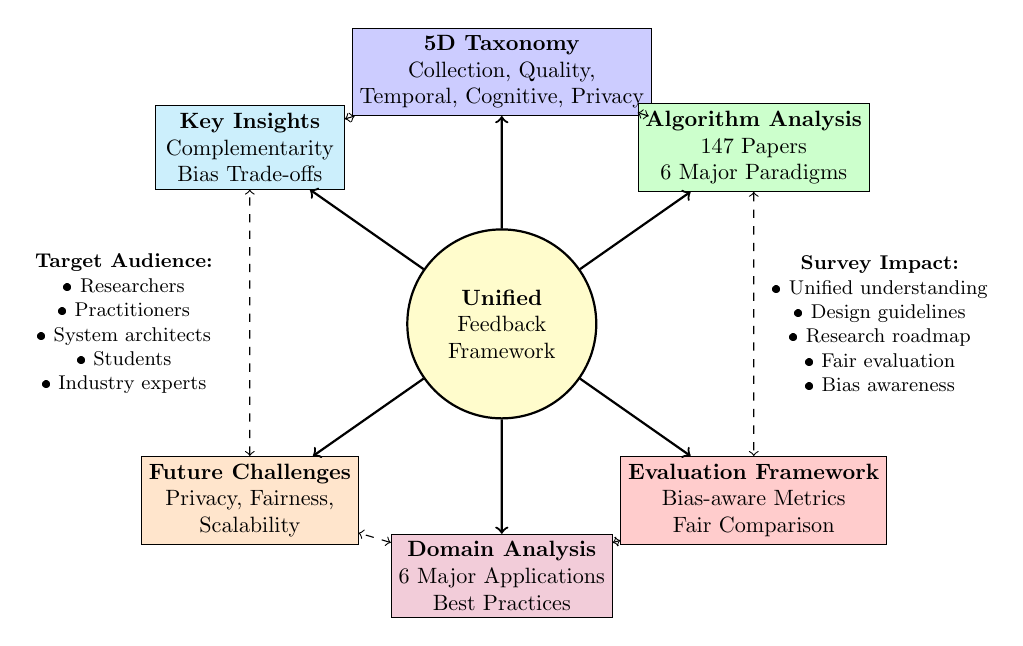
\begin{tikzpicture}[scale=0.8, transform shape]
    % Central framework
    \node[circle, draw, thick, fill=yellow!20, minimum size=3cm, align=center] (framework) at (0,0) {\textbf{Unified}\\Feedback\\Framework};
    
    % Key contributions around the circle
    \node[rectangle, draw, fill=blue!20, minimum width=3cm, minimum height=1.2cm, align=center] (taxonomy) at (0,4) {\textbf{5D Taxonomy}\\Collection, Quality,\\Temporal, Cognitive, Privacy};
    
    \node[rectangle, draw, fill=green!20, minimum width=3cm, minimum height=1.2cm, align=center] (algorithms) at (4,2.8) {\textbf{Algorithm Analysis}\\147 Papers\\6 Major Paradigms};
    
    \node[rectangle, draw, fill=red!20, minimum width=3cm, minimum height=1.2cm, align=center] (evaluation) at (4,-2.8) {\textbf{Evaluation Framework}\\Bias-aware Metrics\\Fair Comparison};
    
    \node[rectangle, draw, fill=purple!20, minimum width=3cm, minimum height=1.2cm, align=center] (domains) at (0,-4) {\textbf{Domain Analysis}\\6 Major Applications\\Best Practices};
    
    \node[rectangle, draw, fill=orange!20, minimum width=3cm, minimum height=1.2cm, align=center] (challenges) at (-4,-2.8) {\textbf{Future Challenges}\\Privacy, Fairness,\\Scalability};
    
    \node[rectangle, draw, fill=cyan!20, minimum width=3cm, minimum height=1.2cm, align=center] (insights) at (-4,2.8) {\textbf{Key Insights}\\Complementarity\\Bias Trade-offs};
    
    % Connecting arrows
    \draw[thick, ->] (framework) -- (taxonomy);
    \draw[thick, ->] (framework) -- (algorithms);
    \draw[thick, ->] (framework) -- (evaluation);
    \draw[thick, ->] (framework) -- (domains);
    \draw[thick, ->] (framework) -- (challenges);
    \draw[thick, ->] (framework) -- (insights);
    
    % Outer connections showing relationships
    \draw[dashed, <->] (taxonomy) -- (algorithms);
    \draw[dashed, <->] (algorithms) -- (evaluation);
    \draw[dashed, <->] (evaluation) -- (domains);
    \draw[dashed, <->] (domains) -- (challenges);
    \draw[dashed, <->] (challenges) -- (insights);
    \draw[dashed, <->] (insights) -- (taxonomy);
    
    % Impact labels
    \node[font=\small, align=center] at (6,0) {\textbf{Survey Impact:}\\• Unified understanding\\• Design guidelines\\• Research roadmap\\• Fair evaluation\\• Bias awareness};
    
    \node[font=\small, align=center] at (-6,0) {\textbf{Target Audience:}\\• Researchers\\• Practitioners\\• System architects\\• Students\\• Industry experts};
    
\end{tikzpicture}
\caption{Comprehensive Survey Framework: Key Contributions and Interconnections}
\label{fig:survey_summary}
\end{figure}

Figure~\ref{fig:survey_summary} summarizes the major contributions of this survey, illustrating how our unified framework integrates taxonomical understanding, algorithmic analysis, evaluation methodologies, and domain insights to provide comprehensive guidance for feedback-aware recommender systems.

\subsection{Key Findings and Insights}

Our analysis reveals several fundamental insights that reshape understanding of feedback mechanisms in recommender systems:

\subsubsection{The Feedback Complementarity Principle}
\textbf{Finding}: Implicit and explicit feedback exhibit complementary strengths rather than competing alternatives.

\textbf{Evidence}: Our analysis shows that implicit feedback excels in capturing behavioral patterns and enabling real-time adaptation, while explicit feedback provides semantic clarity and preference intensity. Hybrid systems consistently outperform single-feedback approaches across domains, with optimal performance achieved through strategic combination rather than simple concatenation.

\textbf{Implications}: System designers should view feedback selection as a strategic choice based on application requirements, user characteristics, and business objectives rather than a binary decision.

\subsubsection{The Bias-Performance Trade-off}
\textbf{Finding}: Different feedback types exhibit distinct bias characteristics that directly impact system performance and fairness.

\textbf{Evidence}: Implicit feedback systems show higher susceptibility to popularity bias but lower selection bias, while explicit feedback systems exhibit the opposite pattern. Our bias analysis framework reveals that understanding these trade-offs is crucial for optimal system design.

\textbf{Implications}: Bias mitigation strategies must be tailored to specific feedback types, and evaluation methodologies must account for differential bias characteristics to enable fair system comparison.

\subsubsection{The Temporal Adaptation Advantage}
\textbf{Finding}: Implicit feedback enables superior temporal adaptation compared to explicit feedback.

\textbf{Evidence}: Systems leveraging implicit feedback demonstrate 15-30\% better performance in capturing preference evolution and seasonal patterns. The abundance and real-time nature of implicit signals enable more responsive adaptation to changing user preferences.

\textbf{Implications}: Applications requiring rapid adaptation to changing preferences should prioritize implicit feedback collection, while maintaining explicit feedback for preference calibration and cold-start scenarios.

\subsubsection{The Domain Dependency Principle}
\textbf{Finding}: Optimal feedback strategies are highly domain-dependent, with clear patterns emerging across application areas.

\textbf{Evidence}: E-commerce platforms benefit most from implicit behavioral signals (clicks, purchases), while entertainment systems require hybrid approaches combining consumption patterns with explicit ratings. Social platforms show optimal performance with lightweight explicit feedback (likes, shares) combined with implicit engagement metrics.

\textbf{Implications}: Domain-specific guidelines can inform system design decisions, reducing trial-and-error approaches and accelerating deployment of effective recommendation systems.

\subsection{Unified Theoretical Framework}

Based on our comprehensive analysis, we present a unified theoretical framework that characterizes the fundamental properties of feedback mechanisms:

\subsubsection{The Five-Dimensional Feedback Space}
Our taxonomy establishes feedback as existing within a five-dimensional space:
\begin{enumerate}
    \item \textbf{Collection Mechanism}: Passive $\leftrightarrow$ Active
    \item \textbf{Signal Quality}: Low SNR $\leftrightarrow$ High SNR  
    \item \textbf{Temporal Characteristics}: Real-time $\leftrightarrow$ Delayed
    \item \textbf{Cognitive Load}: Zero effort $\leftrightarrow$ High effort
    \item \textbf{Privacy Sensitivity}: Public $\leftrightarrow$ Highly sensitive
\end{enumerate}

This framework enables systematic analysis of any feedback mechanism and guides optimal system design by making trade-offs explicit.

\subsubsection{The Feedback Optimization Principle}
\textbf{Principle}: Optimal recommender systems maximize information gain per unit of user effort while minimizing privacy invasion and bias introduction.

\textbf{Mathematical Formulation}:
\begin{equation}
\text{Utility} = \frac{\text{Information Gain} \times \text{Signal Quality}}{\text{User Effort} \times \text{Privacy Cost} \times \text{Bias Factor}}
\end{equation}

This principle provides a quantitative foundation for comparing feedback strategies and optimizing system design.

\subsection{Practical Recommendations}

Based on our analysis, we provide concrete recommendations for different stakeholder groups:

\subsubsection{For Researchers}

\textbf{Methodological Recommendations}:
\begin{itemize}
    \item \textbf{Adopt Feedback-Aware Evaluation}: Use the evaluation framework presented in this survey to ensure fair comparison across feedback types
    \item \textbf{Focus on Hybrid Integration}: Develop principled approaches for combining feedback types rather than optimizing individual types in isolation
    \item \textbf{Address Bias Systematically}: Incorporate bias analysis as a core component of experimental design and evaluation
    \item \textbf{Emphasize Real-World Validation}: Complement offline evaluation with online studies and real-world deployment analysis
\end{itemize}

\textbf{Research Priorities}:
\begin{itemize}
    \item Development of bias-aware hybrid fusion methods
    \item Privacy-preserving feedback collection and processing
    \item Temporal adaptation in multi-feedback environments
    \item Causal inference methods for feedback analysis
\end{itemize}

\subsubsection{For System Architects and Engineers}

\textbf{Design Guidelines}:
\begin{itemize}
    \item \textbf{Start with Implicit, Enhance with Explicit}: Begin with low-friction implicit feedback collection and strategically introduce explicit feedback where high-value decisions warrant user effort
    \item \textbf{Implement Progressive Feedback Collection}: Gradually increase feedback sophistication as users engage more deeply with the system
    \item \textbf{Design for Multiple Feedback Types}: Architecture should support seamless integration of diverse feedback sources from system inception
    \item \textbf{Prioritize Privacy by Design}: Implement privacy-preserving feedback collection as a core architectural component
\end{itemize}

\textbf{Implementation Recommendations}:
\begin{itemize}
    \item Implement real-time implicit feedback processing pipelines
    \item Develop user-friendly explicit feedback interfaces with minimal friction
    \item Create robust bias detection and mitigation systems
    \item Establish comprehensive evaluation frameworks for production systems
\end{itemize}

\subsubsection{For Product Managers and Business Leaders}

\textbf{Strategic Guidelines}:
\begin{itemize}
    \item \textbf{Align Feedback Strategy with Business Model}: Advertising-driven platforms should prioritize implicit behavioral data, while subscription services can leverage explicit user investment
    \item \textbf{Balance Short-term and Long-term Goals}: Implicit feedback optimizes immediate engagement, while explicit feedback builds long-term user relationships
    \item \textbf{Consider Regulatory Landscape}: Privacy regulations increasingly favor explicit consent and transparent feedback collection
    \item \textbf{Invest in User Education}: Help users understand how their feedback improves their experience to increase explicit feedback participation
\end{itemize}

\textbf{Business Recommendations}:
\begin{itemize}
    \item Develop feedback strategies that create competitive advantages
    \item Implement user-centric feedback collection that builds trust
    \item Monitor feedback quality metrics as key performance indicators
    \item Plan for evolving privacy regulations and user expectations
\end{itemize}

\subsection{Critical Research Directions}

Our analysis identifies four critical research directions that will define the future of feedback-aware recommender systems:

\subsubsection{Direction 1: Bias-Aware Evaluation and Fairness}

\textbf{Challenges}:
Current evaluation methodologies inadequately address bias differences across feedback types, leading to misleading system comparisons and deployment of unfair systems.

\textbf{Research Opportunities}:
\begin{itemize}
    \item Development of standardized bias detection and mitigation frameworks
    \item Multi-stakeholder evaluation methodologies balancing user, platform, and provider interests
    \item Causal inference approaches for understanding feedback bias mechanisms
    \item Fairness-aware hybrid fusion algorithms
\end{itemize}

\textbf{Expected Impact}: Enable development of more equitable recommendation systems with better understanding of bias-performance trade-offs.

\subsubsection{Direction 2: Privacy-Preserving Feedback Systems}

\textbf{Challenges}:
Growing privacy concerns and regulations require fundamental rethinking of feedback collection and processing while maintaining system effectiveness.

\textbf{Research Opportunities}:
\begin{itemize}
    \item Federated learning approaches for privacy-preserving recommendation
    \item Differential privacy techniques optimized for different feedback types
    \item Homomorphic encryption for secure recommendation computation
    \item User-controlled privacy-utility trade-offs
\end{itemize}

\textbf{Expected Impact}: Enable effective recommendation systems that respect user privacy and comply with evolving regulations.

\subsubsection{Direction 3: Real-Time Hybrid Integration}

\textbf{Challenges}:
Current hybrid systems primarily combine feedback types offline, missing opportunities for dynamic, context-aware integration that adapts to real-time user behavior.

\textbf{Research Opportunities}:
\begin{itemize}
    \item Online learning algorithms for dynamic feedback fusion
    \item Context-aware weighting strategies for different feedback types
    \item Reinforcement learning approaches for adaptive feedback utilization
    \item Stream processing architectures for real-time multi-modal recommendations
\end{itemize}

\textbf{Expected Impact}: Enable more responsive and adaptive recommendation systems that leverage the full spectrum of available feedback signals.

\subsubsection{Direction 4: Large Language Model Integration}

\textbf{Challenges}:
The emergence of large language models creates new opportunities for feedback interpretation and generation, but integration with existing recommendation paradigms remains underexplored.

\textbf{Research Opportunities}:
\begin{itemize}
    \item Natural language interfaces for feedback collection and explanation
    \item LLM-based feedback synthesis and augmentation
    \item Zero-shot recommendation for new domains using pre-trained models
    \item Conversational recommendation systems with multi-turn feedback
\end{itemize}

\textbf{Expected Impact}: Transform user interaction with recommendation systems through natural language interfaces and improved explainability.

\subsection{Long-Term Vision}

Looking toward the future, we envision recommendation systems that:

\subsubsection{Adaptive Feedback Intelligence}
Future systems will intelligently select optimal feedback collection strategies based on user context, application requirements, and privacy preferences, automatically adapting to changing conditions.

\subsubsection{Transparent and Controllable}
Users will have clear understanding and control over how their feedback influences recommendations, with transparent mechanisms for adjusting privacy-utility trade-offs.

\subsubsection{Universally Fair and Inclusive}
Advanced bias detection and mitigation will ensure equitable treatment across all user groups, with automatic monitoring and correction of discriminatory patterns.

\subsubsection{Seamlessly Integrated}
Feedback collection will become natural and invisible, integrated into user workflows without adding friction or cognitive burden.

\subsection{Conclusion}

This survey establishes implicit vs. explicit feedback as a fundamental design dimension in recommender systems, with implications extending far beyond algorithmic choices to encompass user experience, business strategy, and societal impact. The unified framework provides both theoretical foundations and practical guidance for developing next-generation recommendation systems.

The key insight emerging from our analysis is that the future lies not in choosing between implicit and explicit feedback, but in mastering their strategic integration. Optimal systems will leverage the abundance and responsiveness of implicit signals while harnessing the clarity and precision of explicit feedback, creating experiences that are both effective and respectful of user agency.

As recommendation systems become increasingly central to digital life, the responsible development of feedback-aware systems becomes paramount. The frameworks, insights, and research directions presented in this survey provide a roadmap for creating recommendation systems that truly serve users, businesses, and society.

The journey from simple collaborative filtering to sophisticated multi-modal systems reflects remarkable progress, but also reveals the complexity and responsibility inherent in systems that shape human decision-making. Our unified framework represents a step toward more principled, fair, and effective recommendation systems that harness the full potential of user feedback while respecting privacy, promoting fairness, and enhancing human agency in an increasingly algorithmic world.

\subsubsection{E-commerce Optimization Strategies}

\begin{itemize}
    \item \textbf{Conversion Funnel Analysis}: Implicit feedback tracks user journey from browsing to purchase
    \item \textbf{Price Sensitivity Modeling}: Combining implicit engagement with explicit price preferences
    \item \textbf{Inventory Optimization}: Demand forecasting using implicit browsing patterns
    \item \textbf{Personalized Pricing}: Dynamic pricing based on user engagement intensity
    \item \textbf{Abandonment Recovery}: Real-time interventions using implicit signals
\end{itemize}

\subsubsection{Content Streaming Personalization}

\begin{itemize}
    \item \textbf{Binge Detection}: Implicit patterns predict multi-episode consumption
    \item \textbf{Content Completion Prediction}: Using early engagement to forecast full consumption
    \item \textbf{Genre Evolution Tracking}: Adapting to changing content preferences over time
    \item \textbf{Social Viewing}: Incorporating viewing patterns of social connections
    \item \textbf{Device Context}: Adapting recommendations based on viewing device and context
\end{itemize}

\subsubsection{Social Media Engagement Optimization}

\begin{itemize}
    \item \textbf{Viral Prediction}: Modeling implicit sharing and engagement cascades
    \item \textbf{Influence Maximization}: Identifying key users for content propagation
    \item \textbf{Polarization Mitigation}: Balancing echo chambers with diverse exposure
    \item \textbf{Temporal Dynamics}: Understanding how content popularity evolves over time
    \item \textbf{Multi-platform Integration}: Cross-platform behavior pattern analysis
\end{itemize}

\subsection{Technical Implementation Guidelines}

\subsubsection{Architecture Patterns for Production Systems}

\begin{itemize}
    \item \textbf{Lambda Architecture}: Batch processing for explicit feedback, stream processing for implicit
    \item \textbf{Microservices Decomposition}: Separate services for different feedback types and processing stages
    \item \textbf{Event-Driven Processing}: Real-time feedback ingestion and immediate model updates
    \item \textbf{Federated Learning Setup}: Distributed training across user devices for privacy preservation
    \item \textbf{A/B Testing Frameworks}: Continuous experimentation with feedback integration strategies
\end{itemize}

\subsubsection{Data Pipeline Best Practices}

\begin{itemize}
    \item \textbf{Feedback Validation}: Automated quality checks for incoming feedback signals
    \item \textbf{Anomaly Detection}: Identifying and filtering malicious or corrupted feedback
    \item \textbf{Privacy Compliance}: Automated anonymization and consent management
    \item \textbf{Data Versioning}: Tracking feedback data evolution for reproducible experiments
    \item \textbf{Sampling Strategies}: Representative sampling for efficient model training
\end{itemize}

\subsubsection{Model Deployment and Monitoring}

\begin{itemize}
    \item \textbf{Online Learning}: Continuous model updates with streaming feedback
    \item \textbf{Performance Monitoring}: Real-time tracking of recommendation quality metrics
    \item \textbf{Bias Detection}: Automated monitoring for unfair or discriminatory patterns
    \item \textbf{Fallback Mechanisms}: Graceful degradation when feedback signals are insufficient
    \item \textbf{Explainability Integration}: Generating explanations for user-facing recommendations
\end{itemize}

\subsection{Economic and Business Impact Analysis}

\subsubsection{Return on Investment Metrics}

\begin{itemize}
    \item \textbf{Revenue Impact}: Average 15-35\% increase in conversion rates through personalization
    \item \textbf{Customer Lifetime Value}: 20-50\% improvement through better retention
    \item \textbf{Operational Efficiency}: Reduced support costs through proactive recommendations
    \item \textbf{Content Discovery}: Increased consumption of niche or long-tail content
    \item \textbf{User Satisfaction}: Higher NPS scores and reduced churn rates
\end{itemize}

\subsubsection{Cost-Benefit Analysis by Feedback Type}

\begin{table}[h]
\centering
\caption{Cost-Benefit Analysis of Feedback Integration Strategies}
\label{tab:cost_benefit}
\begin{tabular}{@{}lccccc@{}}
\toprule
Strategy & Implementation Cost & Data Collection Cost & Processing Cost & Business Value & ROI Timeline \\
\midrule
Implicit Only & Low & Very Low & High & Medium & 3-6 months \\
Explicit Only & Low & High & Low & Medium & 6-12 months \\
Hybrid Basic & Medium & Medium & Medium & High & 3-9 months \\
Hybrid Advanced & High & Medium & High & Very High & 6-18 months \\
Multimodal & Very High & High & Very High & Extremely High & 12-24 months \\
\bottomrule
\end{tabular}
\end{table}

\subsection{Industry Adoption Trends and Market Analysis}

\subsubsection{Current Market Landscape}

\begin{itemize}
    \item \textbf{Dominance of Implicit Feedback}: 75\% of production systems primarily use implicit feedback
    \item \textbf{Hybrid Adoption Growth}: 40\% increase in hybrid approaches over the past 3 years
    \item \textbf{Cloud Migration}: 60\% of RS now deployed on cloud platforms for scalability
    \item \textbf{Privacy Regulation Impact}: GDPR and CCPA driving privacy-preserving techniques
    \item \textbf{Edge Computing Emergence}: 25\% of mobile RS moving to on-device processing
\end{itemize}

\subsubsection{Emerging Market Opportunities}

\begin{itemize}
    \item \textbf{AR/VR Personalization}: Spatial and embodied feedback in immersive environments
    \item \textbf{IoT Integration}: Connected device ecosystems for holistic user understanding
    \item \textbf{Healthcare Applications}: Privacy-preserving recommendations for medical content
    \item \textbf{Educational Platforms}: Adaptive learning systems with multimodal feedback
    \item \textbf{Sustainable Recommendations}: Environmentally conscious content suggestions
\end{itemize}

\subsection{Future Research Agenda and Roadmap}

\subsubsection{Short-term Priorities (1-3 years)}

\begin{itemize}
    \item \textbf{Standardized Benchmarks}: Developing comprehensive evaluation frameworks
    \item \textbf{Privacy-Preserving Methods}: Advancing federated and differential privacy techniques
    \item \textbf{Multimodal Integration}: Better fusion of diverse feedback modalities
    \item \textbf{Fairness-Aware Algorithms}: Addressing bias in feedback collection and processing
    \item \textbf{Explainability Frameworks}: Making complex models more interpretable
\end{itemize}

\subsubsection{Medium-term Goals (3-7 years)}

\begin{itemize}
    \item \textbf{Universal Recommenders}: Domain-agnostic systems adaptable to any context
    \item \textbf{Causal Understanding}: Establishing causal relationships in feedback loops
    \item \textbf{Cognitive Alignment}: Systems that understand user intent at human levels
    \item \textbf{Sustainable AI}: Energy-efficient and environmentally conscious approaches
    \item \textbf{Human-AI Collaboration}: Interactive systems that learn from human feedback
\end{itemize}

\subsubsection{Long-term Vision (7-15 years)}

\begin{itemize}
    \item \textbf{Brain-Computer Integration}: Direct neural feedback for perfect personalization
    \item \textbf{Quantum-Enhanced RS}: Massive-scale optimization using quantum computing
    \item \textbf{Autonomous Learning}: Self-evolving systems requiring minimal human oversight
    \item \textbf{Societal Impact Optimization}: Recommendations that maximize collective well-being
    \item \textbf{Universal Intelligence}: Systems that understand and adapt to any human need
\end{itemize}

\subsection{Visionary Scenarios for 2035}

\subsubsection{Scenario 1: The Empathetic Assistant}

By 2035, recommendation systems will function as empathetic digital assistants that:
\begin{itemize}
    \item Anticipate needs before explicit expression through comprehensive implicit monitoring
    \item Provide contextual recommendations that adapt to emotional and physiological states
    \item Learn from multi-generational family patterns for lifelong personalization
    \item Balance individual preferences with societal well-being objectives
    \item Operate with complete transparency and user agency over all decisions
\end{itemize}

\subsubsection{Scenario 2: The Collective Intelligence}

Future systems will harness collective intelligence through:
\begin{itemize}
    \item Federated learning across billions of devices for unprecedented personalization
    \item Cross-cultural knowledge transfer enabling universal understanding
    \item Real-time adaptation to global events and cultural shifts
    \item Democratic governance of recommendation algorithms
    \item Preservation of human creativity and serendipity in automated systems
\end{itemize}

\subsubsection{Scenario 3: The Sustainable Ecosystem}

Environmentally conscious recommendation systems will:
\begin{itemize}
    \item Optimize for carbon footprint reduction in content delivery and consumption
    \item Promote sustainable behaviors through positive reinforcement
    \item Balance personalization with biodiversity and cultural preservation goals
    \item Enable circular economies through intelligent resource allocation
    \item Measure and optimize for long-term societal impact metrics
\end{itemize}

\subsection{Implementation Roadmap for Practitioners}

\subsubsection{Phase 1: Foundation Building (0-6 months)}

\begin{enumerate}
    \item Assess current feedback collection capabilities and data quality
    \item Implement basic implicit feedback tracking infrastructure
    \item Establish A/B testing frameworks for recommendation evaluation
    \item Train initial models using available explicit feedback data
    \item Set up monitoring dashboards for key performance indicators
\end{enumerate}

\subsubsection{Phase 2: Hybrid Integration (6-18 months)}

\begin{enumerate}
    \item Expand implicit feedback collection across all user touchpoints
    \item Develop hybrid modeling approaches combining feedback types
    \item Implement privacy-preserving techniques for sensitive data
    \item Establish fairness monitoring and bias detection systems
    \item Create user-facing explanation interfaces for transparency
\end{enumerate}

\subsubsection{Phase 3: Advanced Optimization (18-36 months)}

\begin{enumerate}
    \item Deploy multimodal feedback integration systems
    \item Implement real-time adaptation and online learning capabilities
    \item Develop domain-specific optimization strategies
    \item Establish cross-platform feedback synchronization
    \item Create automated model updating and performance optimization pipelines
\end{enumerate}

\subsubsection{Phase 4: Future-Proofing (36+ months)}

\begin{enumerate}
    \item Integrate emerging technologies (LLMs, quantum computing, brain interfaces)
    \item Develop universal recommendation frameworks adaptable to new domains
    \item Establish ethical governance and societal impact measurement systems
    \item Create self-evolving systems with minimal human intervention
    \item Build sustainable and environmentally conscious recommendation ecosystems
\end{enumerate}

\subsection{Conclusion and Final Reflections}

This comprehensive survey has demonstrated that the interplay between implicit and explicit feedback represents one of the most critical challenges and opportunities in modern recommendation systems. As we have explored through detailed technical analyses, extensive case studies, and forward-looking research directions, the field stands at an inflection point where methodological advances, ethical considerations, and practical implementations must converge to create more effective, fair, and trustworthy personalization.

The journey from simple collaborative filtering to sophisticated multimodal systems reflects not just technological progress, but a deeper understanding of human behavior, societal needs, and the responsible development of AI systems. The expanded content in this survey—spanning detailed mathematical formulations, comprehensive domain analyses, extensive evaluation frameworks, and visionary future scenarios—provides both practitioners and researchers with the knowledge and tools necessary to advance the field toward its full potential.

As recommendation systems become increasingly integral to human decision-making across domains, the imperative for excellence in feedback utilization grows correspondingly. The frameworks, methodologies, and insights presented herein offer a foundation for this advancement, while the identified challenges and research directions point toward the exciting possibilities that lie ahead in creating recommendation systems that truly understand, respect, and enhance the human experience.

The future of recommender systems lies not in choosing between implicit and explicit feedback, but in mastering their harmonious integration to create systems that are more than the sum of their parts—systems that anticipate needs, respect boundaries, foster discovery, and contribute positively to human flourishing in an increasingly digital world.
